\chapter{Construcción de wavelets}\label{chapter:state-of-the-art}

El objetivo de este trabajo es replicar la DST-II y explorar su comportamiento en el caso de señales de dos 
dimensiones. Sin embargo, antes de hablar de los detalles de este algoritmo, es necesario introducir
algunos conceptos sobre las wavelets y su construcción. En la Sección \ref{wavelet-transform} 
de este capítulo se introducen la definición de wavelet
y de la transformada, tanto continua como discreta y la relación de esta última con los bancos de filtros. Luego, en
la Sección \ref{design-selection-wavelets} se exponen algunos 
de los criterios más usados para caracterizar a las wavelets y ejemplos de wavelets clásicas, para después 
hablar de algunas de las técnicas más recientes usadas en la generación de wavelets adaptadas a datos o problemas
específicos (entre ellas, la DST en sus tres variantes).

\section{Transformada Wavelet Continua }\label{wavelet-transform}

Antes de definir formalmente qué es una wavelet, es necesario definir el espacio de las funciones 
de cuadrado integrable.
Este espacio, denotado por $L^2(\mathbb{R})$ está formado por las funciones $f$ que cumplen \cite{frazier}:

\begin{equation}
	\int_{\mathbb{R}} |f(x)|^2 dx < \infty.
\end{equation}

Sobre este espacio, el producto interno $\langle \cdot,\cdot \rangle$ de $f,g \in L^2(\mathbb{R})$ se define como:
\begin{equation}
	\langle f,g \rangle = \int_{\mathbb{R}} f(x)g^*(x) dx,
\end{equation}
\noindent donde el operador $*$ denota el conjugado complejo.

Una wavelet es una función $\psi \in L^2(\mathbb{R})$ con promedio cero \cite{Mallat2008}:
\begin{equation}
	\int_{-\infty}^{+\infty} \psi(t) dt = 0.
\end{equation}
También se cumple que $\psi$ está normalizada, es decir, $||\psi||=1$. Además, $\psi$ está centrada en la vecindad
$t=0$. A partir de las traslaciones y dilataciones de $\psi$ se puede generar una familia de funciones:

\begin{equation}
	\left\{ \psi_{u,s}(t)= \frac{1}{\sqrt{s}}\psi \left(\frac{t-u}{s}\right) \right\}_{u \in \mathbb{R}, s \in \mathbb{R^+}},
\end{equation}
\noindent donde $u$ es el factor del desplazamiento y $s$ la escala. Estas nuevas funciones $\psi_{u,s}$ siguen estando
normalizadas. Luego, la transformada wavelet continua (TWC) de una función $f$ se define como:

\begin{equation}
	Wf(u,s) = \langle f,\psi_{u,s} \rangle = \int_{-\infty}^{+\infty}  f(t)\frac{1}{\sqrt{s}}\psi^*\left(\frac{t-u}{s}\right) dt.
\end{equation}

Si se define la operación de convolución como:
\begin{equation}
	f*g(x) = \int_{\mathbb{R}} f(x-y)g(x)dy,
\end{equation}
\noindent la TWC también se puede definir de esta forma:

\begin{equation}
	Wf(u,s) = \int_{-\infty}^{+\infty}  f(t)\frac{1}{\sqrt{s}}\psi^*\left(\frac{t-u}{s}\right) dt = f*\bar \psi_s(u),
\end{equation}
\noindent donde $$\bar \psi_s(t)=\frac{1}{\sqrt{s}}\psi^*\left(\frac{-t}{s}\right).$$

El concepto de función de escala también es importante cuando se trata de la transformada wavelet. 
Cuando $Wf(u,s)$ es conocido solamente para valores de $s<s_0$, para recuperar $f$ se necesita información
complementaria correspondiente a $Wf(u,s)$ para $s>s_0$. Por este motivo, se introduce
la función $\phi$, la cual se conoce como la función de escala, porque es la suma de todas las wavelets con
escalas mayores que uno. La función $\phi$ también está normalizada ($||\phi||=1$).

Sea 
\begin{equation}
	\phi_s(t) = \frac{1}{\sqrt{s}}\phi\left(\frac{t}{s}\right),
\end{equation}
\noindent entonces la aproximación de bajas frecuencias de $f$ se define como:

\begin{equation}
	Lf(u,s) = \langle f(t),\frac{1}{\sqrt{s}}\phi\left(\frac{t-u}{s}\right) \rangle = f*\phi_s(u).
\end{equation}


\subsection{Transformada Wavelet Discreta }

Para el caso de las señales discretas, una base wavelet discreta es necesaria. Por esto, primero se requiere
obtener un conjunto discreto de wavelets mediante la discretización de $s$ y $u$. Sea $u=ks$ y $s=a^j$, 
para $k,j \in \mathbb{Z}$ y $a>1$, entonces:

\begin{equation}
	\psi_j[n] = \frac{1}{a^j}\psi\left(\frac{n}{a^j}\right).
\end{equation}

Luego la transformada wavelet discreta (TWD) se define como \cite{Mallat2008}:

\begin{equation}\label{eq:Wf}
	Wf[n,a^j] = \sum_{m=0}^{N-1} f[m] \psi_{j}^*[m-n] = f * \bar \psi_j[n],
\end{equation}

\noindent donde $\bar \psi_j[n] = \psi_j^*[-n]$.

De forma similar, la función de escala se puede definir como:

\begin{equation}
	\phi_j[n] = \frac{1}{a^j}\phi\left(\frac{n}{a^j}\right),
\end{equation}

donde $\bar \phi_j[n] = \phi_j^*[-n]$. Luego, 

\begin{equation}\label{eq:Lf}
	Lf[n,a^j] = \sum_{m=0}^{N-1} f[m] \phi_{j}^*[m-n] = f \circledast \bar \phi_j[n],
\end{equation}

\noindent es una aproximación de $f$, pero sin los componentes de alta frecuencia, tal y como ocurría en el caso
de la TWC. 
Cuando $a=2$, se le conoce como transformada diádica \cite{Mallat2008}.

\subsection{Bancos de filtros}\label{filter-banks}

El uso de filtros en el procesamiento de señales es bastante amplio e incluso es anterior a 
la gran incursión de las wavelets en esta área. 
Sin embargo, ambos están relacionados y la TWD se puede definir en términos de filtros.

Un filtro es un operador lineal invariante en el tiempo. Actúa sobre un vector de entrada $x$.
El vector de salida $y$  es la convolución de $x$ con un vector fijo $h$, tal y como se muestra
a continuación \cite{Gilbert95} :

\begin{equation}
	y[n] = \sum_{k} h[k]x[n-k] = h * x.
\end{equation}

El vector $h$ contiene los coeficientes del filtro. En el caso de los filtros digitales, los 
coeficientes $h(n)$ vienen en tiempos discretos $t=nT$, donde $T$ es el período de muestreo. 
Si la entrada es un vector $x=(\cdots,0,1,0,\cdots)$, donde tiene una unidad de impulso en el tiempo cero,
es decir, $x[n-k]=0$, para $n \neq k$, entonces la suma de la convolución tiene un solo término, que sería
$h[n]$. Esta salida $y[n]=h[n]$, es la respuesta en el tiempo $n$ a la unidad de impulso
$x[0]=1$. La respuesta de impulso del filtro es $h[0],h[1],\cdots,h[N]$ \cite{Gilbert95}.

Si la respuesta de impulso del filtro es de duración finita, porque se hace cero en tiempo finito, entonces
el filtro se conoce como filtro de respuesta finita al impulso (FIR, en inglés).

En el dominio de las frecuencias, la convolución con el vector $h$, se convierte en una multiplicación. La 
acción de los filtros en el tiempo y la frecuencia son los fundamentos sobre los que el procesamiento de señales
está construido \cite{Gilbert95}.

Un banco de filtros es un conjunto de filtros. El banco de análisis, por lo general, tiene dos filtros, 
de paso bajo (\textit{lowpass}) y de paso alto (\textit{highpass}). Estos separan la señal 
de entrada en bandas de frecuencias. Normalmente, no es necesario
conservar la salida entera de los filtros de análisis y solamente se mantienen los componentes pares de la salida
de los filtros. Este proceso se llama submuestreo o decimación (\textit{downsampling}). 

En el marco de las wavelets ortogonales, el algoritmo de descomposición y reconstrucción se puede definir
en términos de operaciones con filtros. Las siguientes ecuaciones \cite{Mallat2008}:

\begin{equation}
	a_j[n] = \langle f,\phi_{j,n} \rangle,
\end{equation}

\begin{equation}
	d_j[n] = \langle f,\psi_{j,n} \rangle,
\end{equation}

\noindent son las proyecciones de $f$ sobre $\{\phi_{j,n}\}_{n\in \mathbb{Z}}$ y $\{\psi_{j,n}\}_{n\in \mathbb{Z}}$, 
respectivamente. El primer vector $a$ representa los coeficientes de aproximación de la función $f$,
y $d$ los de detalle. Estos coeficientes $d_j$ y $a_j$ corresponden a (\ref{eq:Wf}) y (\ref{eq:Lf}) 
respectivamente. 

Sean los filtros 

\begin{equation}
	h[n] = \langle \frac{1}{\sqrt{2}} \phi\left(\frac{t}{n}\right), \phi(t-n) \rangle,
\end{equation}

\begin{equation}
	g[n] = \langle \frac{1}{\sqrt{2}} \psi\left(\frac{t}{n}\right), \phi(t-n) \rangle,
\end{equation}

\noindent o de forma equivalente,

\begin{equation}
	\phi(t) = \sum_n \sqrt{2}h[n]\phi(2t-n),
\end{equation}

\begin{equation}
	\psi(t) = \sum_n \sqrt{2}g[n]\phi(2t-n).
\end{equation}

Las siguientes fórmulas muestran como calcular los coeficientes de la TWD, partiendo de los filtros 
$h$ y $g$, y es conocido como algoritmo de Mallat:

\begin{equation}\label{eq:mallat-aprox}
	a_{j+1}[p] = \sum_{-\infty}^{+\infty} h[n-2p]a_j[n] = (a_j * \bar h)[2p],
\end{equation}

\begin{equation}\label{eq:mallat-details}
	d_{j+1}[p] = \sum_{-\infty}^{+\infty} g[n-2p]d_j[n] = (d_j * \bar g)[2p],
\end{equation}

\noindent donde el operador $\bar x$ sobre $h$ y $g$ indican el reverso del filtro.

Las fórmulas (\ref{eq:mallat-aprox}) y (\ref{eq:mallat-details}) corresponden al banco de filtro para la
descomposición o análisis de la señal. 

En el caso del banco de filtro para el proceso inverso, es decir, la reconstrucción o síntesis de la señal a 
partir de los coeficientes, se tiene la siguiente fórmula:

\begin{equation}
	a_j[p] = \sum_{n= -\infty}^{+\infty} h[p-2n]a_{j+1}[n] + \sum_{n= -\infty}^{+\infty}g[p-2n]d_{j+1}[n],
\end{equation}

\noindent o de forma equivalente, 

\begin{equation}
	a_j[p] = ( \check a_{j+1} * h )[p] + ( \check d_{j+1} * g )[p],
\end{equation}

\noindent donde el operador $\check x$ sobre $a_j$ y $d_j$ denota la señal insertando ceros en los índices impares
(\textit{upsampled}).

\begin{figure}\label{fig:dwt-filterbanks-1D}
	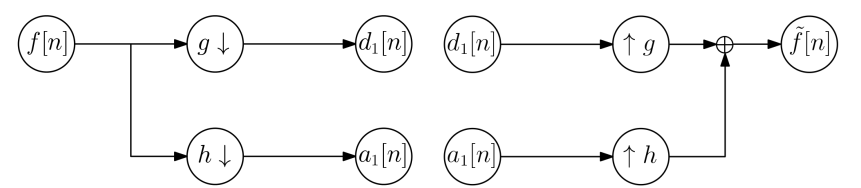
\includegraphics[scale=0.5]{Graphics/dwt-filterbanks-1D.png}
	\caption{Representación gráfica del proceso de descomposición (análisis) y reconstrucción (síntesis) de la señal $f$. La $\uparrow$ corresponde a la operación de \textit{upsampling} y la $\downarrow$ a la de \textit{downsampling} (Tomado de \cite{Recoskie2018} pág. 25).}\label{fig:dwt-filterbanks-1D}
\end{figure}

La Figura \ref{fig:dwt-filterbanks-1D} muestra una representación gráfica de ambos bancos de filtros, es decir, 
el proceso cómputo de la transformada y de su inversa. Empezando por $a_0[n] = f[n]$, se procede a calcular recursivamente
los coeficientes de aproximación y de detalle, tal y como se describe en (\ref{eq:mallat-aprox}) y (\ref{eq:mallat-details}),
respectivamente. Este algoritmo es bastante eficiente, pues tiene un costo computacional de $O(n)$, donde $n$
es el tamaño de la señal. 

Una de las propiedades de este algoritmo es la invertibilidad, es decir, después de haber sido deconstruída, el proceso
de reconstrucción permite obtener la señal original. La principal propiedad necesaria en un banco de filtro 
para que se cumpla lo anterior es la propiedad de reconstrucción perfecta. 

\subsection{TWD para dos dimensiones}\label{section:dwt-2d}

La transformada wavelet discreta se puede extender de varias formas para el caso de imágenes.
En la descomposición estándar la transformada es aplicada a todas las columnas para todas las escalas
y luego a todas las filas del resultado. En la descomposición no estándar la transformada se calcula en cada
eje por separado, es decir, primero se realiza la transformada a las filas y luego a las columnas del resultado. 
Esta forma de descomposición es la más usada y se denomina producto tensorial \cite{WaveletVariants2D}.

En el caso 1D, se calculan dos compenentes de la señal en cada iteración del algoritmo (paso alto y
paso bajo). En el caso 2D, para la descomposición no estándar, se calculan cuatro componentes. $LR$ y $LC$ son 
el resultado del filtro de paso bajo
sobre las filas y las columnas, respectivamente. De forma similar, se definen $HR$ y $HC$, pero para el caso
del filtro de paso alto. En cada iteración del algoritmo de la TWD, se obtienen las siguientes componentes:

\begin{itemize}
	\item Coeficientes de aproximación LL: $LC(LR(X))$
	\item Coeficientes de detalle horizontal LH: $LC(HR(X))$
	\item Coeficientes de detalle vertical HL: $HC(LR(X))$ 
	\item Coeficientes de detalle diagonal HH: $HC(HR(X))$
\end{itemize}

\begin{figure}
	\begin{center}
		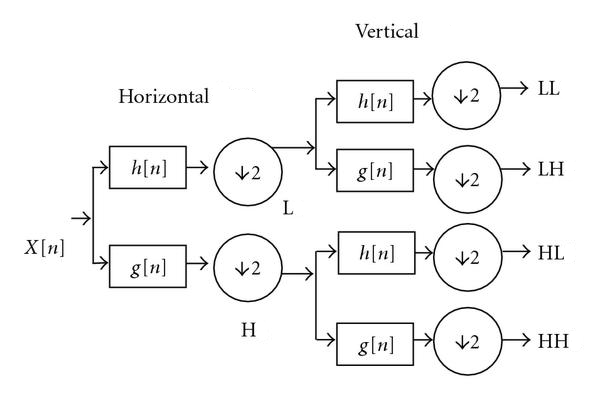
\includegraphics[scale=2]{Graphics/dwt-2D.png}
		\caption{Representación gráfica del proceso de descomposición (análisis) de la señal bidimensional $X$. La $\downarrow$ corresponde a la operación de \textit{downsampling}.}\label{fig:dwt-2D}
	\end{center}
\end{figure}

\noindent donde $X$ es una señal discreta de dos dimensiones. Los tres componentes calculados haciendo uso del 
filtro de paso alto son considerados coeficientes de detalle, y el otro restante, corresponde a los coeficientes de aproximación. 
Los grupos de coeficientes de
detalles, corresponden cada uno a una orientación: horizontal, vertical y diagonal. Cada uno responde a cambios en su
respectiva dirección. Al igual que en el caso unidimensional, se hace un submuestreo sobre la señal original
en cada convolución con los filtros. La Figura \ref{fig:dwt-2D} representa gráficamente
el proceso de obtención de la TWD para el caso de una señal bidimensional.

En el aspecto de la complejidad computacional, el algoritmo es $O(n^2)$, teniendo como entrada
una señal bidimensional $X$ de dimensiones  $n \times n $. Sin embargo, sigue siendo polinomial 
con respecto a la cantidad de elementos de la señal.

\section{Selección y diseño de wavelets}\label{design-selection-wavelets}

\begin{figure}[!h]
	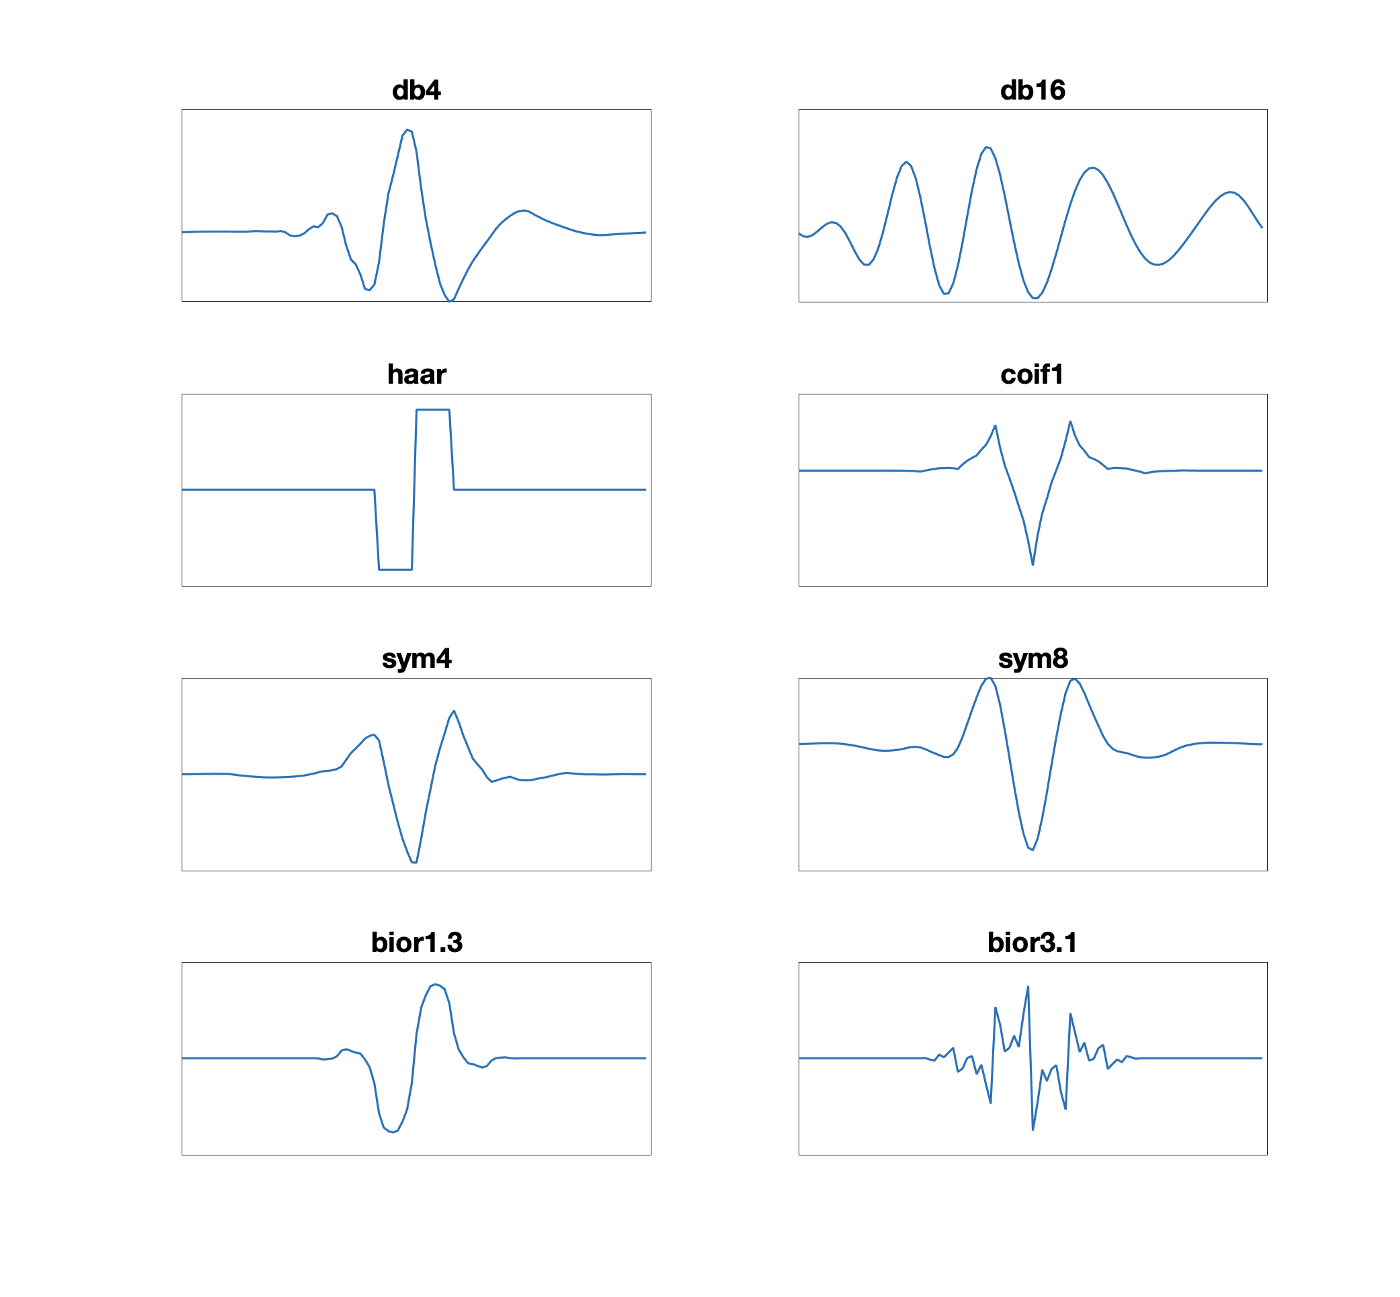
\includegraphics[width=15cm,height=10cm]{Graphics/wavelets.png}
	\caption{Algunos de ejemplos de wavelets.}\label{fig:wavelets}
\end{figure}

Una de las ventajas que tienen las wavelets con respecto a la transformada de Fourier es que 
existe una gran diversidad de wavelets, cada una con sus características, que 
la convierten en la mejor para ciertos escenarios. En la Figura \ref{fig:wavelets} se muestra algunas de las
más conocidas. Sin embargo, dicha variedad constituye también un obstáculo.
Encontrar la wavelet que mejor se adapta al problema en cuestión puede ser un proceso bastante complejo.

\subsection{Familias de wavelets}\label{wavelets-families}

Desde la aparición de la base Haar a principios del siglo pasado, y la explosión de las wavelet en los 
años 1980s, numerosos tipos de wavelet han aparecido en la literatura y softwares especializados en el 
procesamiento de señales. 

Generalmente, los criterios usados para caracterizar a las wavelet son \cite{misiti2007wavelets}:
\begin{enumerate}
	\item El soporte de las funciones $\psi$ y $\phi$ , o su velocidad de convergencia a  cero cuando tienden a 
		infinito.
	\item La simetría, que es útil para evitar desfasajes.
	\item El número de momentos nulos (\textit{vanishing moments}), propiedad de gran importacia en la compresión.
	\item La existencia de la función escala $\phi$.
	\item La ortogonalidad y biortogonalidad.
\end{enumerate}

Muchas aplicaciones de las wavelets explotan su habilidad para aproximar de forma eficiente ciertos tipos de 
funciones. Tal es el caso de la compresión de datos y la reducción y/o eliminación de ruido.
Los momentos nulos o \textit{vanishing moments} son las propiedades de las wavelets que 
hacen posible la representación de funciones suaves con un pequeño número de coeficientes.

Se dice que una wavelet $\psi$ tiene $p$ momentos nulos si:
\begin{equation}
	\int_{-\infty}^{\infty} t^k\psi(t)dt= 0 , \forall 0 \leq k < p.
\end{equation}
Esto significa que la wavelet $\psi$ es ortogonal a cualquier polinomio de grado $p-1$.
Se cumple que si $f$ es regular y $\psi$ tiene suficientes momentos nulos, entonces los coeficientes 
son pequeños, lo cual se puede aprovechar para compresión de datos.

La construcción de wavelets ortogonales con soporte compacto permite el uso del algoritmo de Mallat.
Las  wavelets de Daubechies \cite{daubechies1992}, denotadas por $dbN$ ($N$ indica el orden de la wavelet),
son una de las más conocidas de este tipo. La $db1$, o wavelet Daubechies de primer orden es la wavelet Haar.
Excepto para esta wavelet, las demás de la familia ($dbN$, con $N>1$) no tienen una expresión explícita de la 
función. Además de la ortogonalidad, esta familia tiene las siguientes características:

\begin{enumerate}
	\item El tamaño del soporte de $\phi$ y $\psi$ es $2N-1$, donde $N$ es el número de momentos nulos de $\psi$.
	\item Las $dbN$, exceptuando la wavelet de Haar ($db1$), son asimétricas.
	\item La regularidad aumenta con el orden.
\end{enumerate}

Otra familia de wavelets bastante conocida son las Symlets ($symN$). Estas wavelets son una modificación en la forma
de construir las $dbN$, con el objetivo de lograr simetría.

Las Coiflets ($coifN$) \cite{daubechies1992} son otra familia con propiedades bastante interesantes. Al igual que las dos familias de 
wavelets mencionadas anteriormente, la wavelet $\psi$ de $coifN$ posee $2N$ momentos nulos, pero la función escala
$\phi$ tiene $2N-1$ momentos nulos. Las dos funciones $\phi$ y $\psi$ tienen soporte de longitud $6N-1$.

Las wavelets biortogonales extienden la familia de las ortogonales. De la teoría de filtros se sabe que
la simetría y la reconstrucción perfecta no son compatibles (exceptuando a la wavelet Haar)
cuando se usan el mismo par de filtros, para los procesos 
de descomposición y de reconstrucción de una señal \cite{misiti2007wavelets}. Para poder contrarrestar esta dificultad se usan un par de
wavelets. Una para cada proceso. De este modo es posible buscar las propiedades más deseadas para cada uno de
los procesos por separado en cada wavelet.

Una de las técnicas más conocidas para la construcción de bases wavelet es el método \textit{lifting}, presentado
por primera vez en \cite{lifting}. En este trabajo se propone una nueva generación de wavelets, más general, 
que no son necesariamente traslaciones 
o dilataciones, pero que siguen gozando de todas las beneficiosas propiedades de las wavelets 
de primera generación.
A estas nuevas wavelets se les llama de segunda generación. 

En el esquema \textit{lifting},
un filtro finito, llamado \textit{lifting step}, es usado para 
generar un nuevo par de filtros a partir de otro par existente. Múltiples \textit{lifting steps} pueden ser aplicados
consecutivamente. Dos propiedades interesantes de este esquema son la preservación de la biortogonalidad
y que cualquier wavelet con filtros finitos puede se expresada como una secuencia de \textit{lifting steps}.

\subsection{Wavelets adaptadas a los datos}\label{adapted-wavelets}

En la gran mayoría de las aplicaciones, la selección de las wavelets es fundamental. Se han hecho varios trabajos
para encontrar metodologías y criterios para seleccionar las mejores wavelets en ciertas aplicaciones \cite{ngui2013} \cite{doi:10.1177/14759217211010261}.
Sin embargo, en ocasiones, las wavelets predefinidas que se tienen a mano, no son la mejor opción.
La construcción de una wavelet que posea las propiedades que serían idóneas para un problema puede ser una
vía de solución. Esta es una línea que se ha trabajado en el área de las wavelets, proponiéndose varias
técnicas para la obtención de nuevas funciones basadas en los datos.

El esquema \textit{lifting} ha sido usado en conjunción con otros algoritmos para obtener wavelets 
optimizadas para un conjunto de datos.
En \cite{Grasemann2004} se propone un método basado en un algoritmo genético evolutivo. Este algoritmo codifica las wavelets
como una secuencia de \textit{lifting steps}, para luego ir seleccionando y generando los mejores 
candidatos.

En el caso multidimensional también se han hecho estudios para la obtención de wavelets optimizadas para el problema.
En \cite{Gouze2004} se propone un método para el diseño de filtros \textit{lifting} multidimensionales adaptados a las señales, y  
su aplicación en la compresión de imágenes.

En trabajos más recientes, se han incorporado técnicas de aprendizaje automático para la construcción de filtros.
En \cite{Recoskie2018} se propone un método usando redes neuronales artificiales para aprender funciones 
wavelets directamente de los datos. Esta técnica se aplica al caso unidimensional y se extiende también a otras 
dimensiones.

El Análisis de Componentes Principales (PCA, por sus siglas en inglés) es usado en \cite{floryan}, para la construcción de una base wavelet llamada por los autores como \textit{data-driven wavelet decomposition}
(DDWD). En este método, se impone muy poca estructura a la base que se crea, y cualquier estructura adquirida durante su construcción
es proveniente del conjunto de datos.

La detección de patrones usando wavelets construidas a partir de un patrón es otro de los enfoques trabajados en las wavelets adaptadas a datos.  
En \cite{Mesa2005AdaptedWF} se propone una variante del método de \textit{lifting} para la detección de patrones en señales unidimensionales.
Partiendo de un patrón, se diseñan a través del esquema de \textit{lifting} unas wavelets, y proponen un procedimiento
de detección dividido en tres etapas. Un algoritmo de optimización basado en mínimos cuadrados es usado en \cite{rpeak}
para diseñar una wavelet, que es luego usada en la TWC para detectar un patrón específico. 
Técnicas como las  anteriores pueden ser aplicadas en diversos campos. Por ejemplo, en \cite{Layouni2017} 
se usan wavelets adaptadas a 
patrones para la detección de defectos en tuberías de gas y petróleo.

La DST \cite{Guido2008} es otra de las técnicas que se basa en la construcción de una wavelet (en este caso se le llama \textit{shapelet})
a partir de un patrón. La DST añade al análisis temporal y de frecuencias, el de forma. El concepto de \textit{shapelet}
está inspirado en el de \textit{Spikelet} y \textit{Speechlet}, pero a diferencia de estos si se logra  la condición
de reconstrucción perfecta. Basado en el concepto de \textit{shapelet} el trabajo \cite{lifting-shapelet}, pero usando
el esquema \textit{lifting} para la construcción de los filtros. 

En \cite{Guido2018} se hacen modificaciones a la DST para crear una segunda versión: DST-II. Esta última
comparte muchas de las características de la primera versión, excepto por las condiciones 
de detección (\textit{matching}).
Esta nueva variante añade las condiciones antes mencionadas de forma tal que el producto escalar inherente al algoritmo
de Mallat durante el cálculo de la transformada sea $0$.

Recientemente, en \cite{Guido2021}, el mismo autor propone una mejora a las dos versiones anteriores de la 
DST e introduce la tercera generación: DST-III. Esta variante, a diferencia de las dos anteriores, permite 
la creación de \textit{shapelets} casi simétricas. 


